\pdfinfo{
    /Author (Zanella Matteo)
    /Title (Example title)
    /Keyword ()
}

% Libraries
\documentclass[a4paper,twoside,12pt]{report}
\usepackage[utf8]{inputenc}
\usepackage[english]{babel}
\usepackage{fancyhdr}
\usepackage{sectsty}
\usepackage[inner=3cm,top=2cm,bottom=2cm,outer=2cm]{geometry}
\usepackage{setspace}
\usepackage[hang,small,sf,font=small, labelfont=bf]{caption}
\usepackage{subcaption}
\usepackage[usenames]{color}
\usepackage{xcolor}
\usepackage{colortbl}
\usepackage{tocloft}
\usepackage[a-1b]{pdfx}
\usepackage{hyperref}
\usepackage{tabto}
\usepackage{mathtools}
\usepackage{bbold}
\usepackage{wrapfig}
\usepackage[]{mdframed}
\usepackage{amsmath}
\usepackage{amsthm}
\usepackage{amssymb}
\usepackage{cases}
\usepackage{indentfirst}
\usepackage{afterpage}
\usepackage{placeins}
\usepackage{csquotes}

%images
\usepackage{graphicx}
\graphicspath{ {./images/} }

%tikz
\usepackage{tikz}
\usetikzlibrary{arrows.meta}

%pseudocode
\usepackage{algorithm}
\usepackage{algpseudocode}


\DeclarePairedDelimiter\floor{\lfloor}{\rfloor}
\DeclarePairedDelimiter\ceil{\lceil}{\rceil}

\setlength{\arrayrulewidth}{1pt}
\newcommand\blankpage{%
    \null
    \thispagestyle{empty}%
    \addtocounter{page}{-1}%
    \newpage}

% Mandatory settings
\onehalfspacing
\hypersetup{
    colorlinks,
    citecolor=black,
    filecolor=black,
    linkcolor=black,
    urlcolor=black
}

% Subsections
\renewcommand{\cftpartleader}{\cftdotfill{\cftdotsep}} % for parts
\renewcommand{\cftchapleader}{\cftdotfill{\cftdotsep}} % for chapters
\renewcommand{\cftsecleader}{\cftdotfill{\cftdotsep}} % for sections

% Bibliography
\usepackage[sorting=none]{biblatex}
\addbibresource{bibl.bib}

% Start document
\begin{document}
\begin{titlepage}
    \centering
    \begin{center}

        \includegraphics[height=0.13\textheight]{logo_unipd.png}
        \hfill
        \includegraphics[height=0.13\textheight]{logo_dei.png}
        \newline
        \newline

        \vspace{0.8cm}
        \textsc{\LARGE Universit\`{a} degli Studi di Padova}\\
        \vspace{1.6cm}
        \textsc{\large 	School of Engineering Department of Information Engineering}\\
        \vspace{0.4cm}

        \textsc{\large Master Degree in Computer Engineering}\\
        \vfill
        { \LARGE \bfseries Example of a Title}\\
        \vspace{1cm}

        \textbf{\large Example of a Subtitle}\\
        \vfill

        \textit{\large Supervisor:} \hfill \textit{\large Candidate:}\\
        \textsc{\large Professor} \hfill \textsc{Zanella Matteo}\\
        \textsc{Università di Padova} \hfill \textsc{Badge\_number}\\

        \vfill

        Academic Year 2024/2025

        \vfill

    \end{center}
\end{titlepage}

\pagenumbering{roman}
\thispagestyle{empty}
\clearpage{\pagestyle{plain}\cleardoublepage}
    
\clearpage\null\newpage

% Abstract
\newcommand\summaryname{Abstract}
\newenvironment{Abstract} {
    \begin{center}%
    \bfseries{\summaryname} \end{center}
}

\vspace*{50px}

\begin{Abstract}
    \begin{center}
        This is an example of an abstract.
    \end{center}
\end{Abstract}

\afterpage{\blankpage}

% Index
\clearpage{\pagestyle{plain}\cleardoublepage}
\tableofcontents
%\listoffigures
%\listoftables

\clearpage{\pagestyle{plain}\cleardoublepage}
\pagenumbering{arabic}

% Chapter 1
\clearpage{\pagestyle{plain}\cleardoublepage}
\chapter{Introduction}
This is an example of a chapter\dots

\section{Section 1.1}
\subsection{Subesction 1.1.1}
Write something here...

\section{Math equations examples}

\begin{numcases}
  \displaystyle \min\,\sum_{e\in E}c_ex_e\\
  \displaystyle \sum_{e\in\delta(h)} x_e = 2 \quad \forall \ h\in V\label{HamiltCyc}
  \\
  \displaystyle \sum_{e\in\delta(S)} x_e\leq |S|-1 \quad \forall \ S\subset V : v_1 \in S\label{SEC}
  \\
  \displaystyle 0\leq x_e\leq1 \quad\mbox{integer} \quad \forall \ e\in E
\end{numcases}\\
Constraints \ref{HamiltCyc} impose that every node of the graph must be touched by exactly two edges of the cycle. This group of contraints alone isn't enough to guarantee to find a valid Hamiltonian Cycle: we could find lots of isolated cycles.

\newpage

\section{Pseudocode examples}

\begin{algorithm}
    \caption{Greedy algorithm for the TSP}
    \hspace*{\algorithmicindent} \textbf{Input} Starting node $s\in V$, Set of nodes $V$\\
    \hspace*{\algorithmicindent} \textbf{Output} List of $n\coloneq|V|$ nodes forming an Hamiltonian Cycle, Cost of the cycle
    \begin{algorithmic}

        \State $\mbox{cycle} \gets [s]$
        \State $\mbox{cost} \gets 0$
        
        \For{$i=0 \mbox{ to } n-2$}
            \State $\mbox{next} \gets \mbox{argmin}_{v}{\{c_{cycle[i], v}\;|\;v\not\in \mbox{cycle}\}}$
            \State $\mbox{cost}\gets\mbox{cost}+c_{cycle[i], next}$
            \State $\mbox{cycle}[i+1]\gets\mbox{next}$
        \EndFor
        \State $\mbox{cost}\gets\mbox{cost}+c_{cycle[n-1],s}$\\\\

        \Return cycle, cost
    \end{algorithmic}
\end{algorithm}

\section{Graphs examples}

\begin {center}
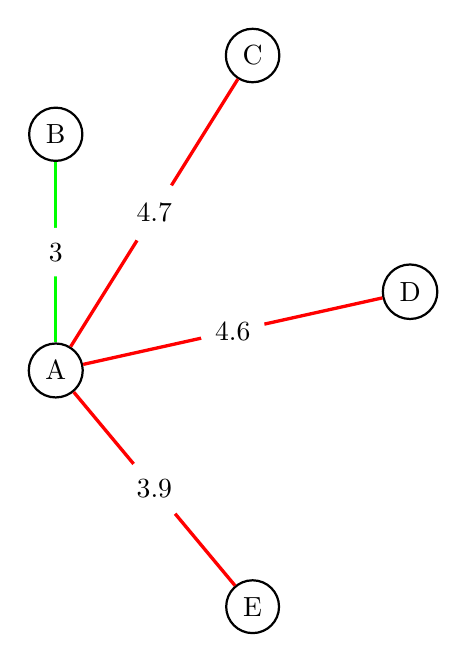
\begin{tikzpicture}
\begin{scope}[every node/.style={circle,thick,draw}]
    \node (A) at (0,0) {A};
    \node (B) at (0,3) {B};
    \node (C) at (2.5,4) {C};
    \node (D) at (4.5,1) {D};
    \node (E) at (2.5,-3) {E};
\end{scope}

\begin{scope}[every node/.style={fill=white,circle},
              every edge/.style={draw=red,very thick}]
    \path [-] (A) edge[draw=green] node {$3$} (B);
    \path [-] (A) edge node {$4.7$} (C);
    \path [-] (A) edge node {$4.6$} (D);
    \path [-] (A) edge node {$3.9$} (E);
    %\path [->] (B) edge[bend right=60] node {$1$} (E); 
\end{scope}
\end{tikzpicture}
\end{center}

\subsection{Example of citations}
This is a citation to Croes \cite{Croes1958AMF}

% Chapter 2
\clearpage{\pagestyle{plain}\cleardoublepage}
\chapter{Other Chapter}
\input{chapters/otherchapter}

\afterpage{\blankpage}
    
% Bibliography
\printbibliography

\end{document}